\documentclass{report}
\usepackage{amsmath}
\usepackage{tabularx}
\usepackage{graphicx}


\begin{document}
\title{Clay-Wolkin Fellowship ISP: Mid-Year Report}
\author{Nick Draper, Christine Goins, Kaveh Pezeshki, Zunyan Wang, Nancy Wei}
\date{November 2017}
\maketitle

\tableofcontents
\listoffigures
\listoftables

\begin{abstract}
	\label{abstract}
\end{abstract}

\chapter{Introduction}

\chapter{Project Goals}
	\section{Constraints}
	\section{Hardware Specification}

\chapter{Background Information}
	\section{Image Signal Processing}
		\subsection{Typical ISP Pipelines}
	\section{Image Recognition via CNN}
	
\chapter{Microarchitecture Specifications}

\chapter{ISP Pipeline Testing}
	\section{Testing Goals}
	In order to establish a pipeline specification for the ISP, it was first necessary to discover what pipeline steps were necessary to achieve adequate machine learning performance, and furthermore, what algorithms were readily available, and easy to implement in hardware, to accomplish these steps. Our required statistic was 90\%+ recognition through all image sets.
	\section{Background}
		\subsection{RAW Conversion}
		In industry, tools such as Adobe Photoshop and Lightroom are often used to edit and convert RAW image formats to standardized formats such as PNG and JPG\footnote{https://digital-photography-school.com/raw-workflow-a-pros-approach/}. However, these products are 'black boxes' and therefore inadequate for the Fellowship's approach to optimizing an ISP for machine learning.
		
		The team therefore investigated the open-source tools UFraw\footnote{http://ufraw.sourceforge.net/} and DCraw \footnote{https://www.cybercom.net/~dcoffin/dcraw/}. While both tools are open-source and provide image conversion and editing capabilities, UFraw provides a powerful and user-friendly wrapper to the DCraw engine. These tools provided a simple way to fine-tune and convert RAW images for machine learning. 
		
		Research on the image quality - machine learning performance correlation already exists\footnote{https://arxiv.org/pdf/1604.04004.pdf}, and indicates that image deviations that can be compensated for in post-processing have substantial impact on recognition rate. The team therefore decided to proceed to test image optimization via UFraw and DCraw.
		\subsection{Metric Calculation}
		In order to judge the efficacy of image optimization, it was first necessary to establish a metric. Focusing on the Inception-V3 image recognition model, trained on ImageNet\footnote{http://www.image-net.org/} and implemented on Google's Tensorflow CNN framework\footnote{https://www.google.com/url?sa=t\&rct=j\&q=\&esrc=s\&source=web\&cd=1\&ved=0ahUKEwiLjZT008LXAhXoqlQKHXgJB0YQFggoMAA\&url=https\%3A\%2F\%2Fwww.tensorflow.org\%2F\&usg=AOvVaw0TGZBeXHx2CVPI2FiDZclR}, the team decided on a simple binary calculation scheme.
		
		Each image set would focus on a specific keyword, with images of the keyword's subject as well as a distribution of images of related and unrelated entities. The metric would be equal to:
		
		\footnotesize
		\begin{equation*}
			\text{metric}=\frac{\text{Number of correct top-5 positive identifications}}{\text{number of images}} + \frac{\text{Number of correct negative identifications}}{\text{number of images}}
		\end{equation*}
		\normalsize
		
		This calculation, as well as an automated image loading and output parsing script, are present in a set of Python scripts. These are available at a Github repository\footnote{https://github.com/Arcturus314/tensorflow\_loader} as well as in Appendix C.
	\section{Image Set Acquisition}
		\subsection{Image Set 1: Cats}
		The initial keyword chosen was 'cat'. This was due to the large proportion of cats and related cat breeds in the ImageNet database\ref{http://image-net.org/synset?wnid=n02127808}, as well as similar quadripedal animals. These characteristics of the ImageNet database would provide a large amount of granularity in the Inception-V3 output. This granularity would allow for a greater level of fine-tuning in ISP pipeline optimization.
		
		There is an animal shelter near Harvey Mudd College, Priceless Pet Rescue\cite{http://pricelesspetrescue.org/}. The initial image set was composed of 179 RAW images of cats and dogs under CFL-lit conditions. There were 32 dogs and 51 cats in this image set. Images were taken in simultaneous RAW-JPG mode with a Canon Rebel t30i, at 5184x3465 pixel resolution.
		
		Images were also taken of dogs and other shelter animals to provide a negative reference. A few example images, processed through the camera pipeline, can be seen in Figure \ref{set1}.
		
		\begin{figure}[h]
			\begin{center}
				\caption{Example Images from Set 1}
				\label{set1}
				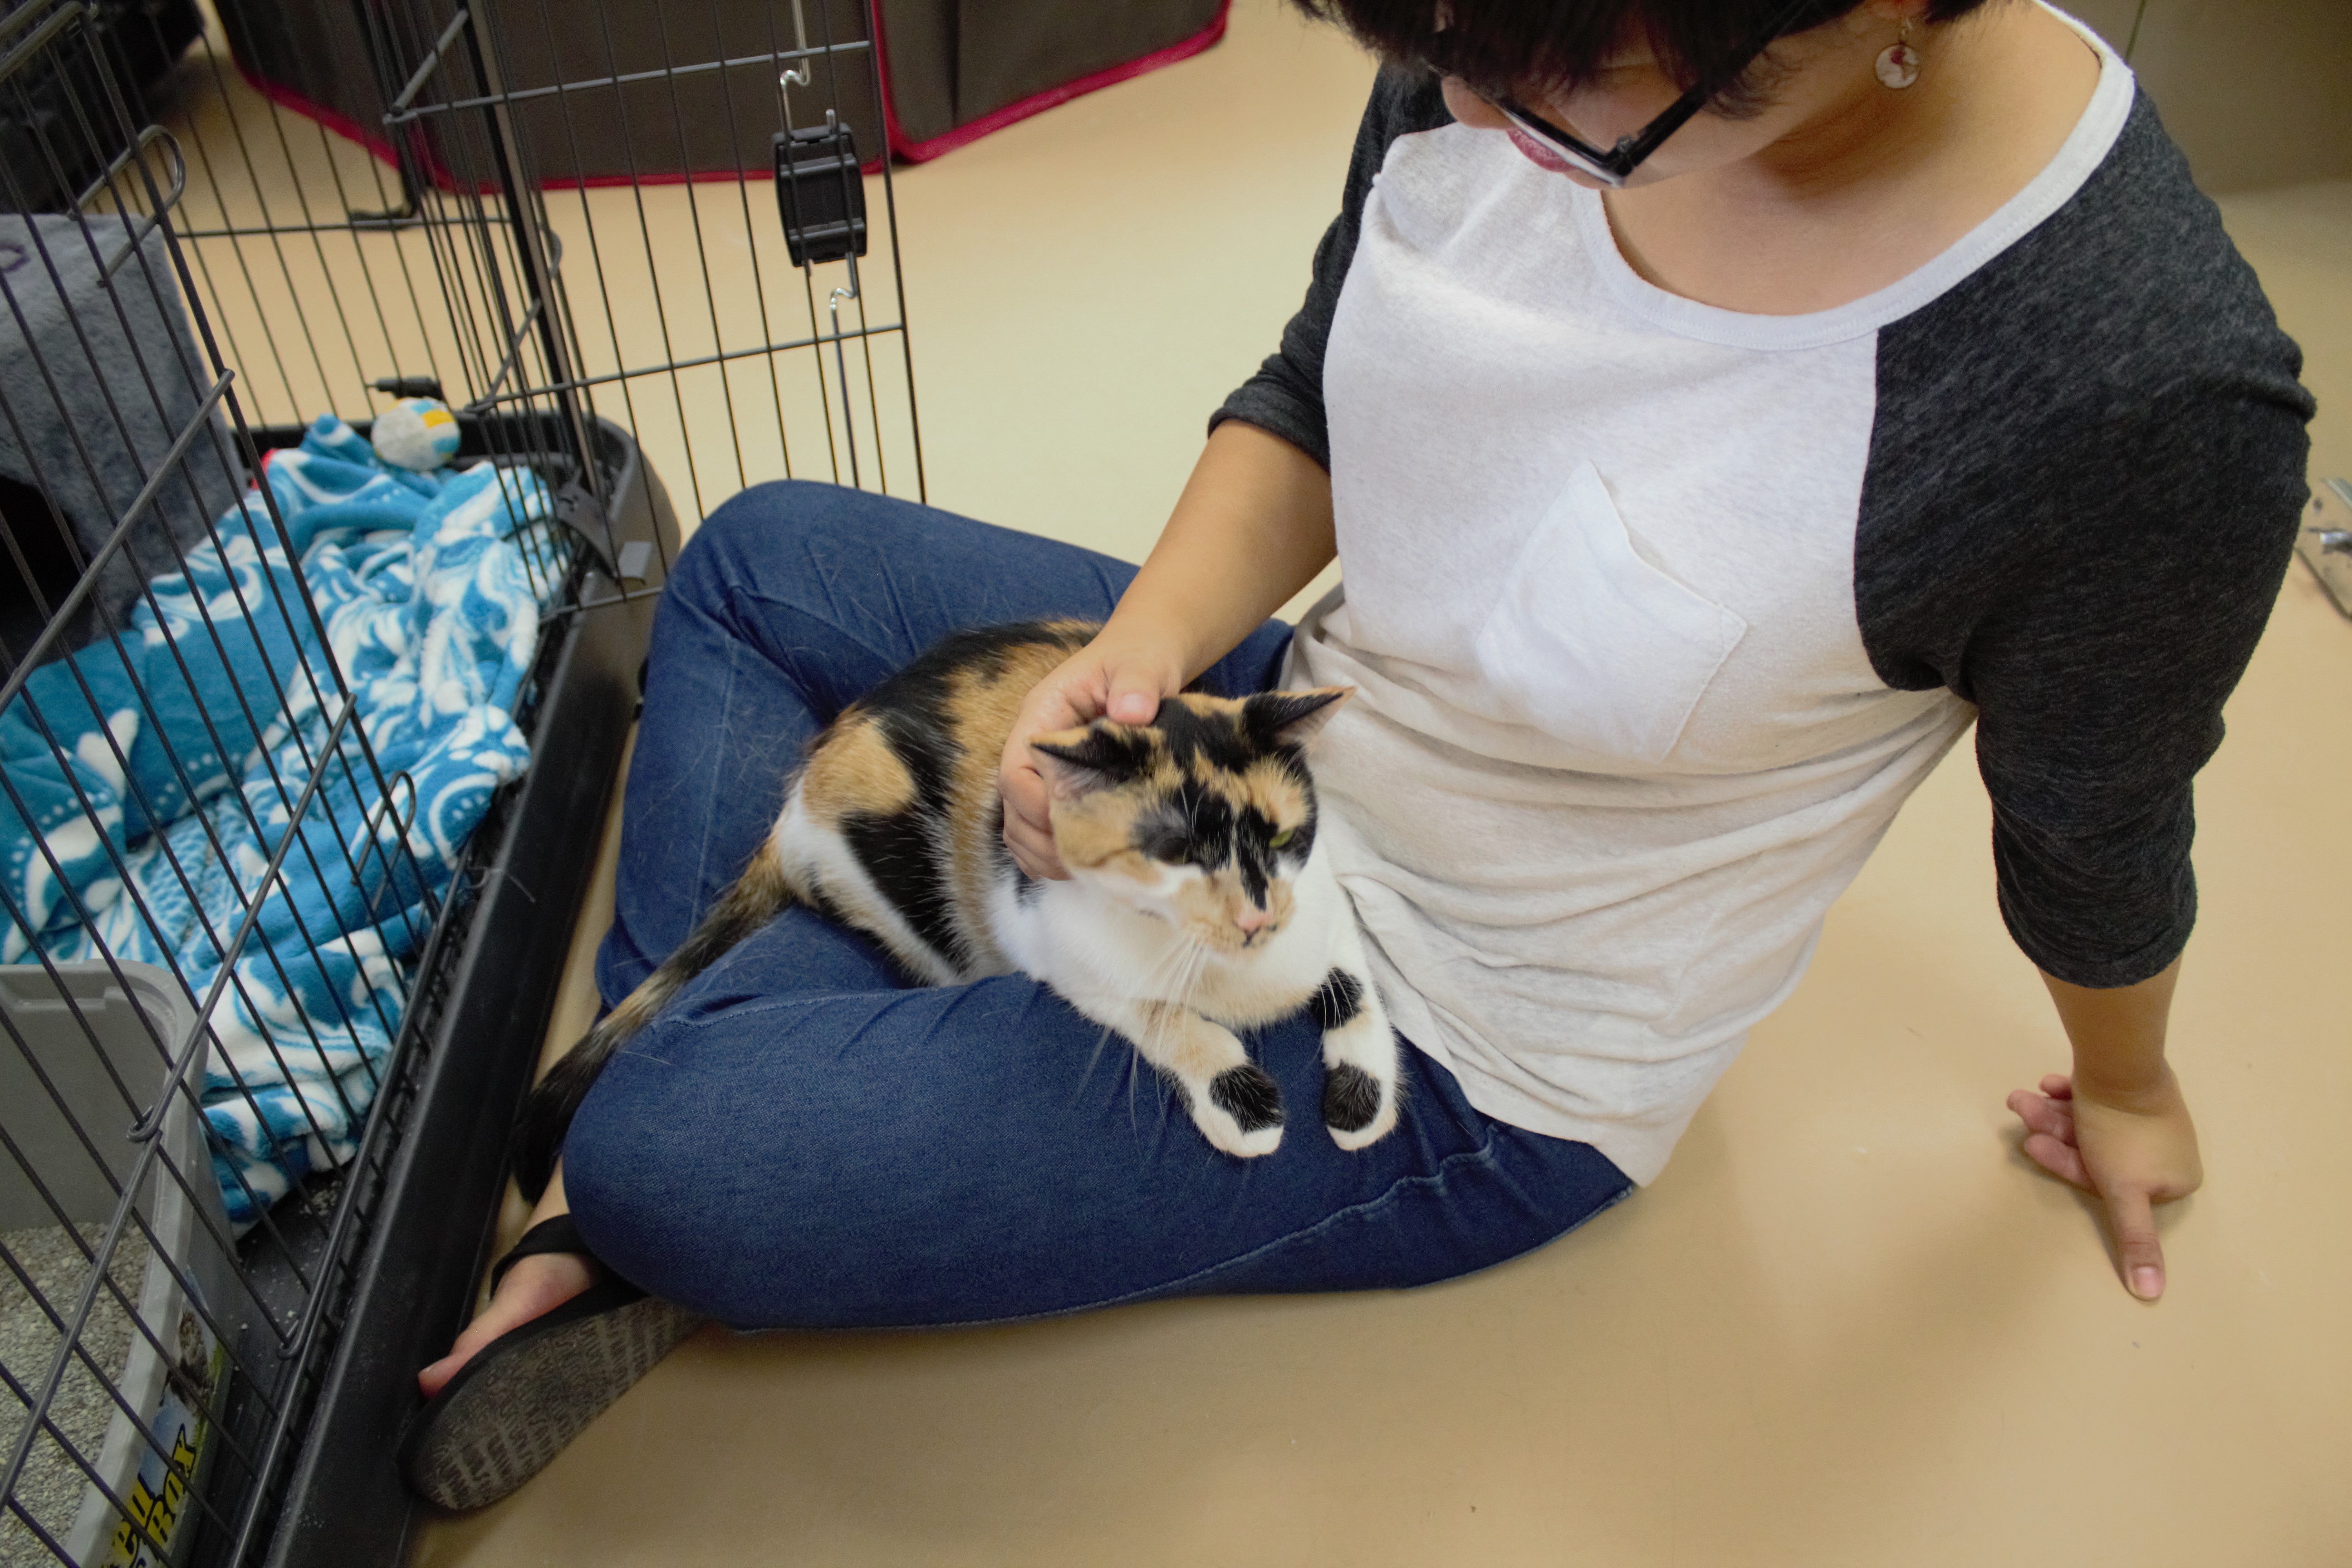
\includegraphics[width=8cm]{set1_cat1.JPG}
				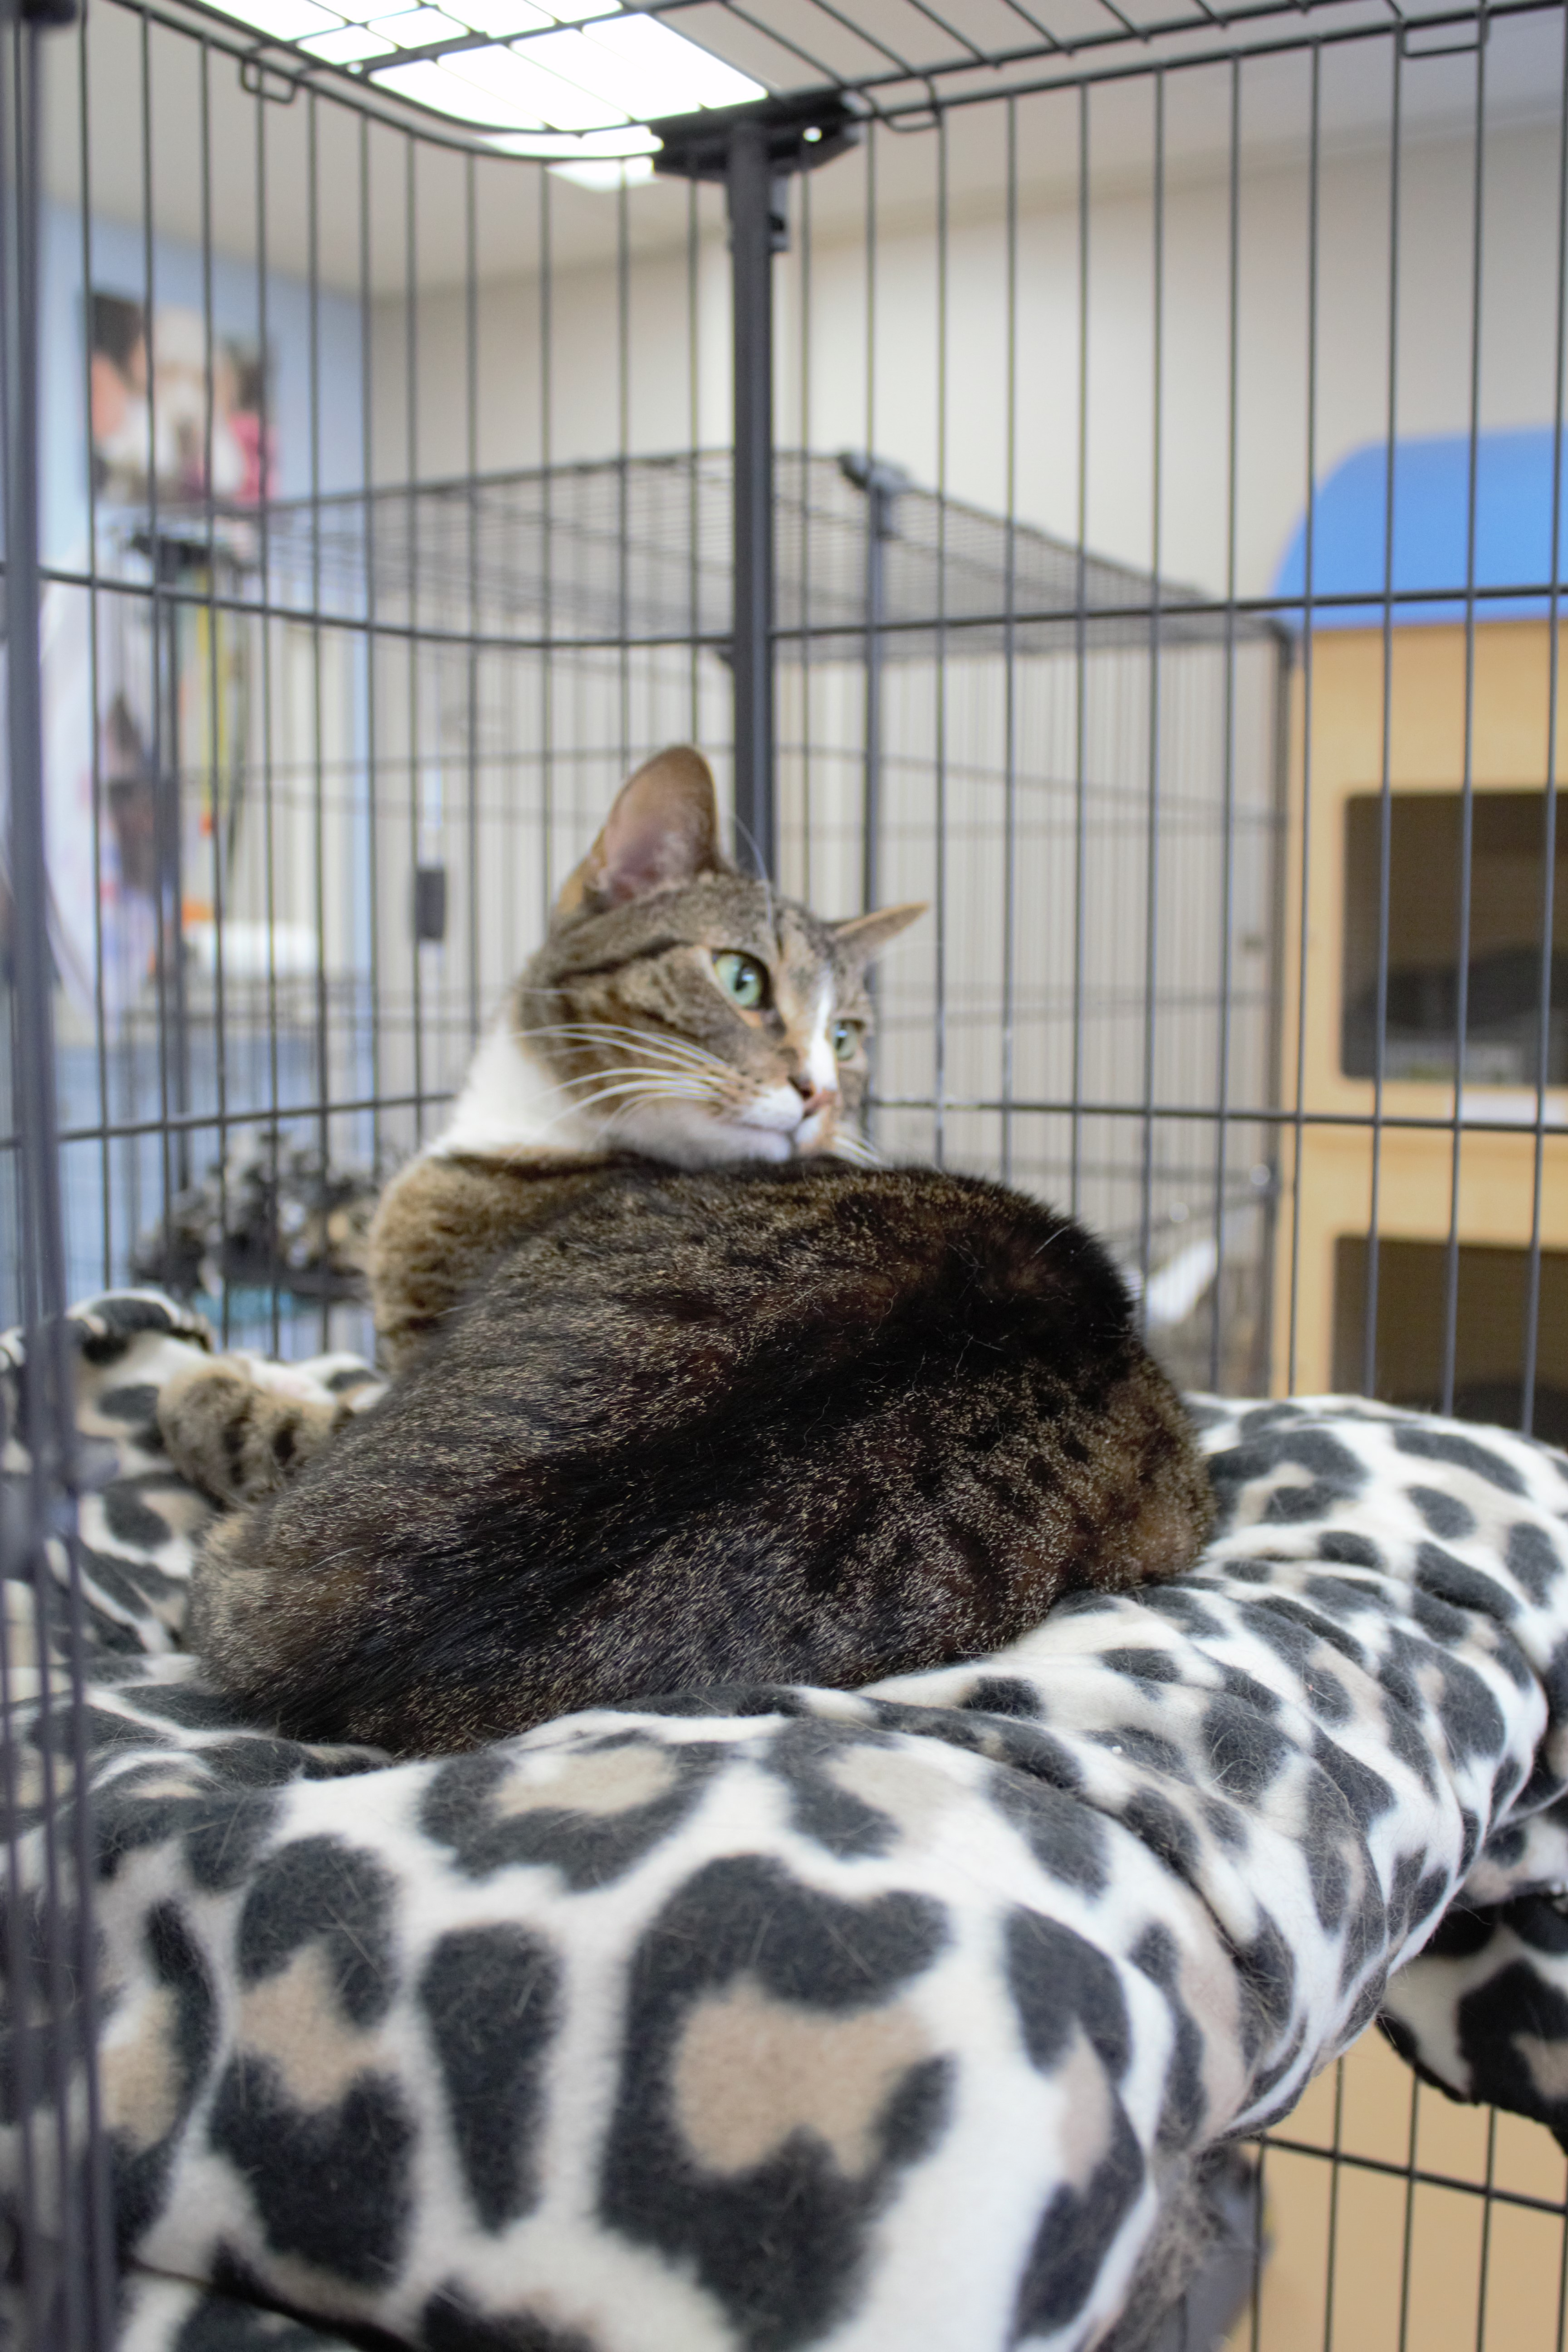
\includegraphics[width=8cm]{set1_cat2.JPG}
				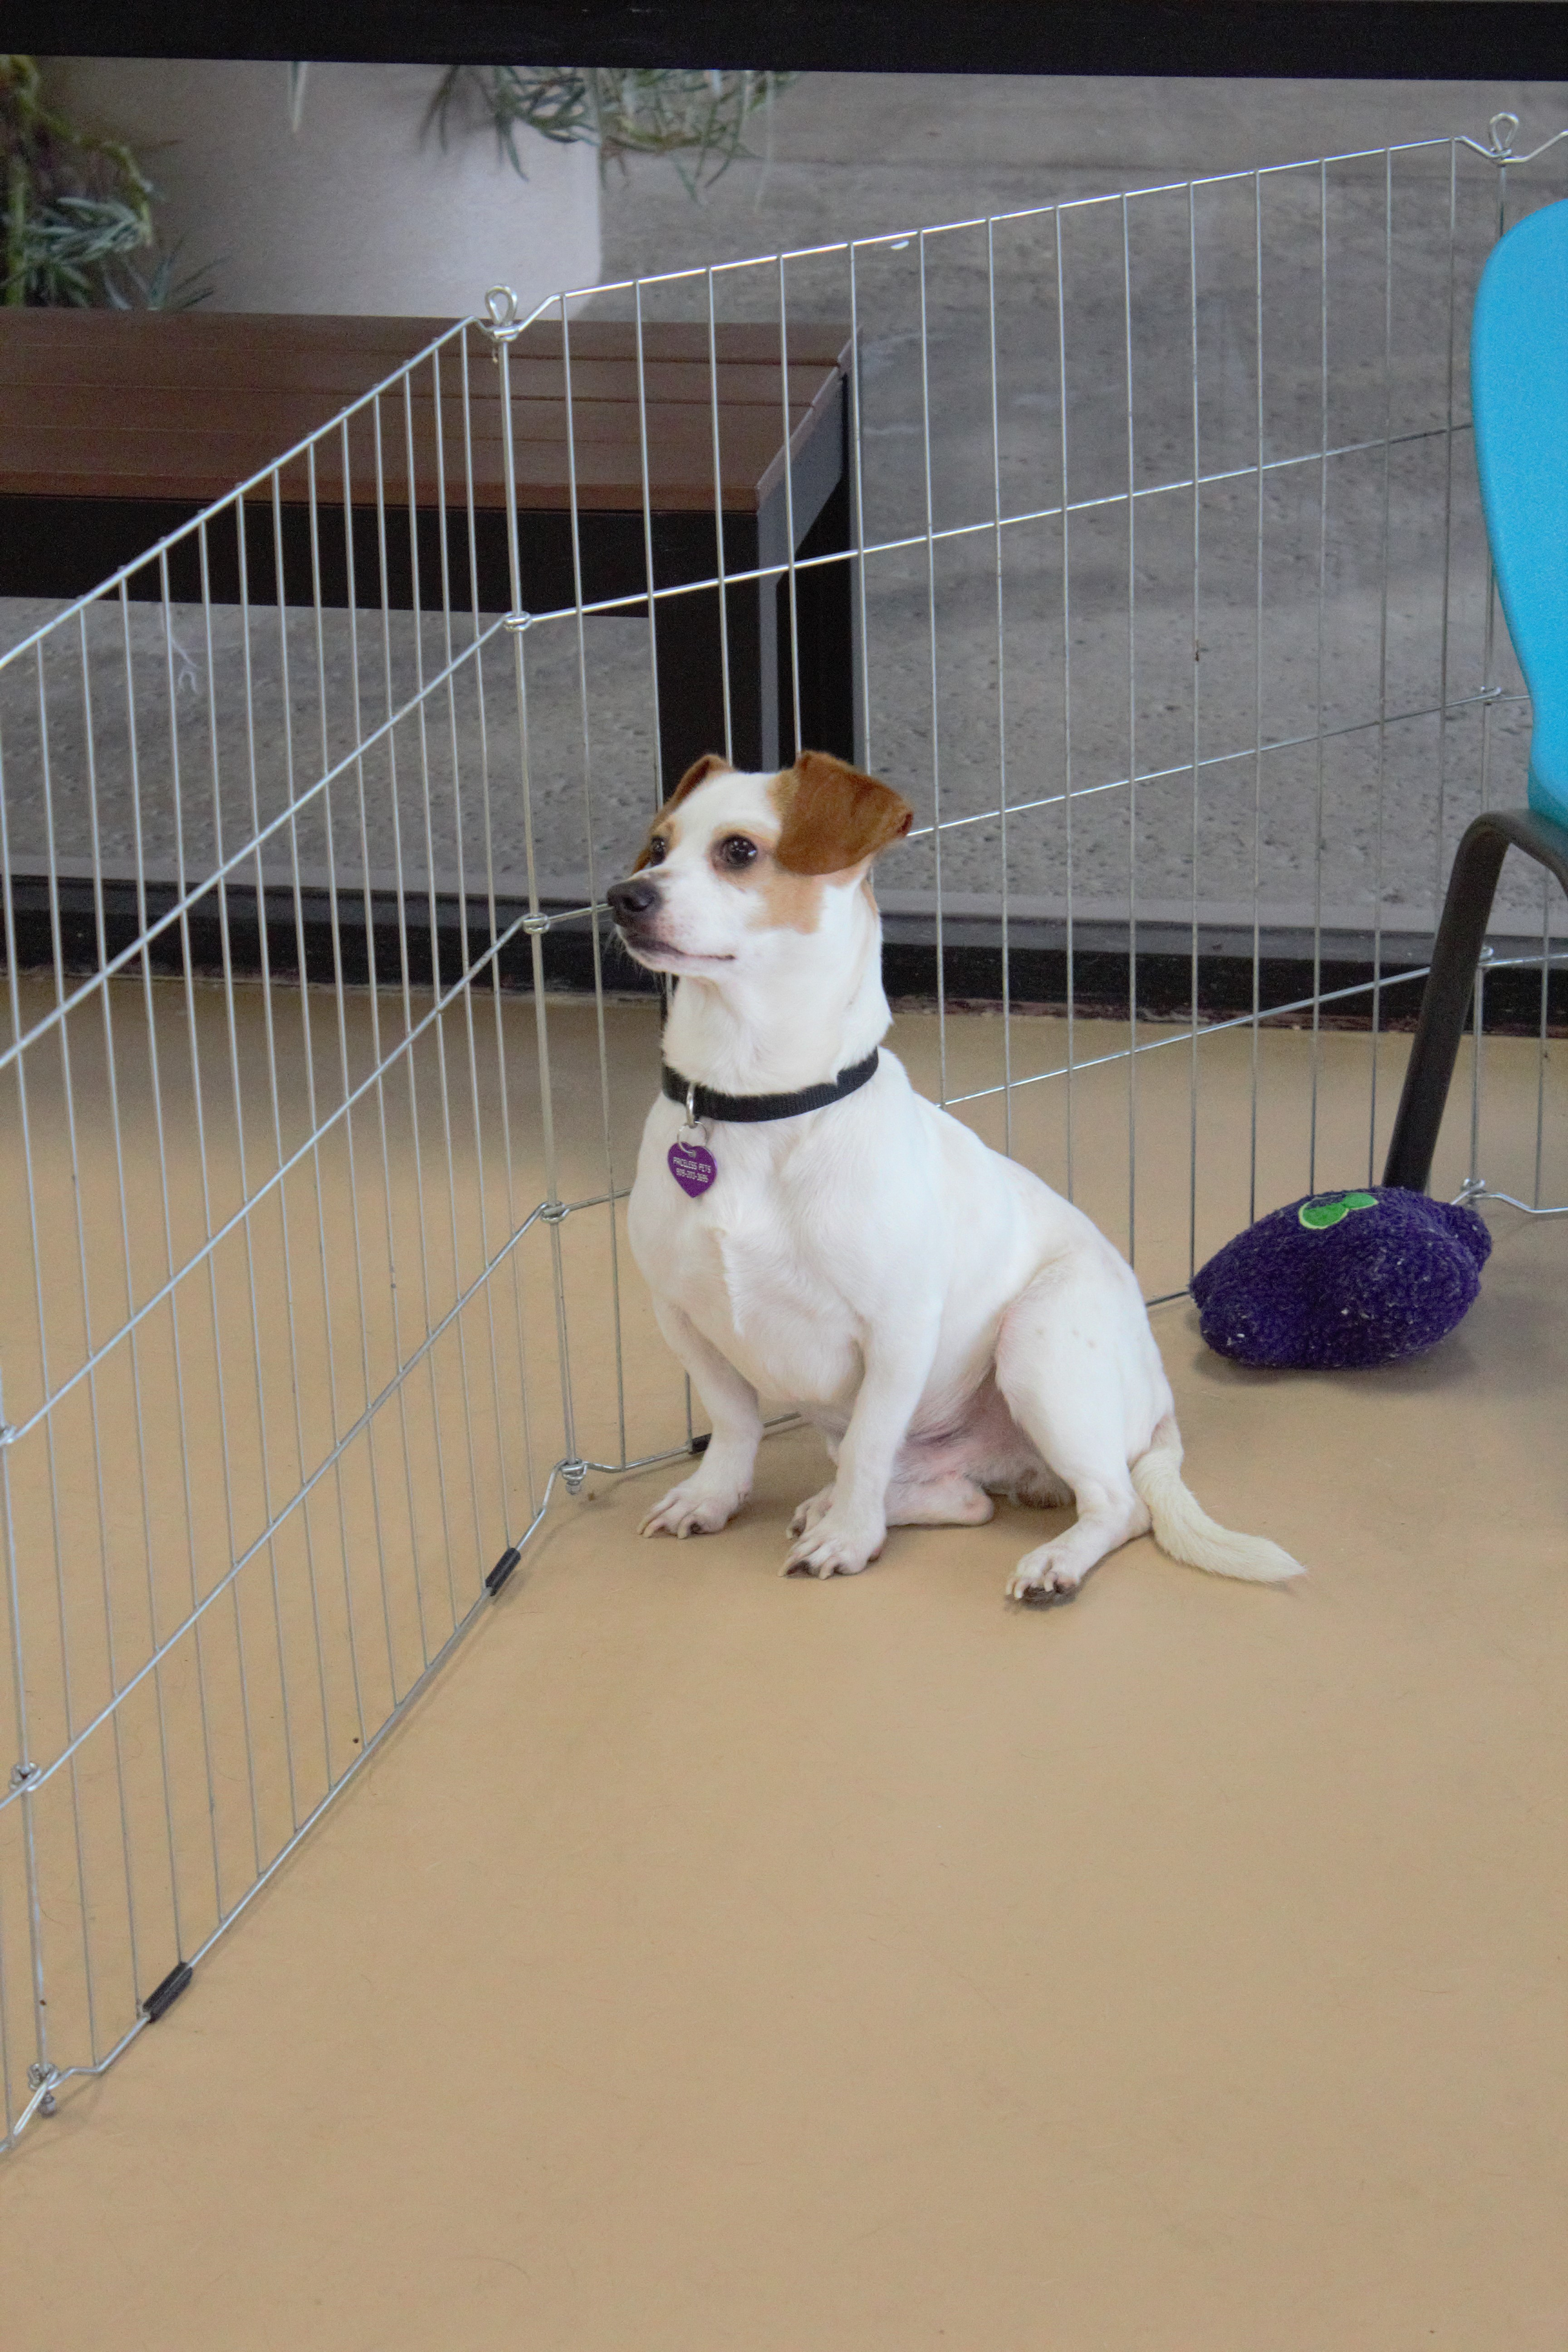
\includegraphics[width=8cm]{set1_dog.JPG}
			\end{center}
		\end{figure}
			
		\subsection{Image Set 2: Cats}
		Realizing that a set of images taken under optimal, well-lit, conditions are likely not representative of images in potential applications of the team's ISP, the team elected to take another set of images at the Priceless Pet Rescue. There were 102 images of cats and 58 images of dogs in this image set for a total of 160 images. Pictures were again taken in simultaneous RAW-JPG mode on a Canon Rebel t30i, except with unoptimal ISO, shutter speed, camera shake, and other parameters.
		
		As before, non-cat images of dogs and other animals were included in the set. Example images can be seen in Figure \ref{set2}. The image quality degradations are immediately clear from these examples.

		\begin{figure}[h]
			\begin{center}
				\caption{Example Images from Set 2}
				\label{set2}
				\includegraphics[width=8cm]{set2_cat1.PNG}
				\includegraphics[width=8cm]{set2_cat2.PNG}
				\includegraphics[width=8cm]{set2_dog.PNG}
			\end{center}
		\end{figure}		
		
		\subsection{Image Set 3: Squash}
		The third and final image set was taken with an unrelated subject --squash-- to help ensure that identification rates were not directly correlated with the cat subject. This image set was taken in simultaneous RAW-JPG mode on a Canon Eos 80D, under outdoor nighttime conditions. Negative samples were of street signs, food products, and other similar objects. There were 29 images of pumpkins of the 102 images in this set.
		
		As before, example images are given in Figure \ref{set3}.
		
	\begin{figure}[h]
		\begin{center}
			\caption{Example Images from Set 3}
			\label{set3}
			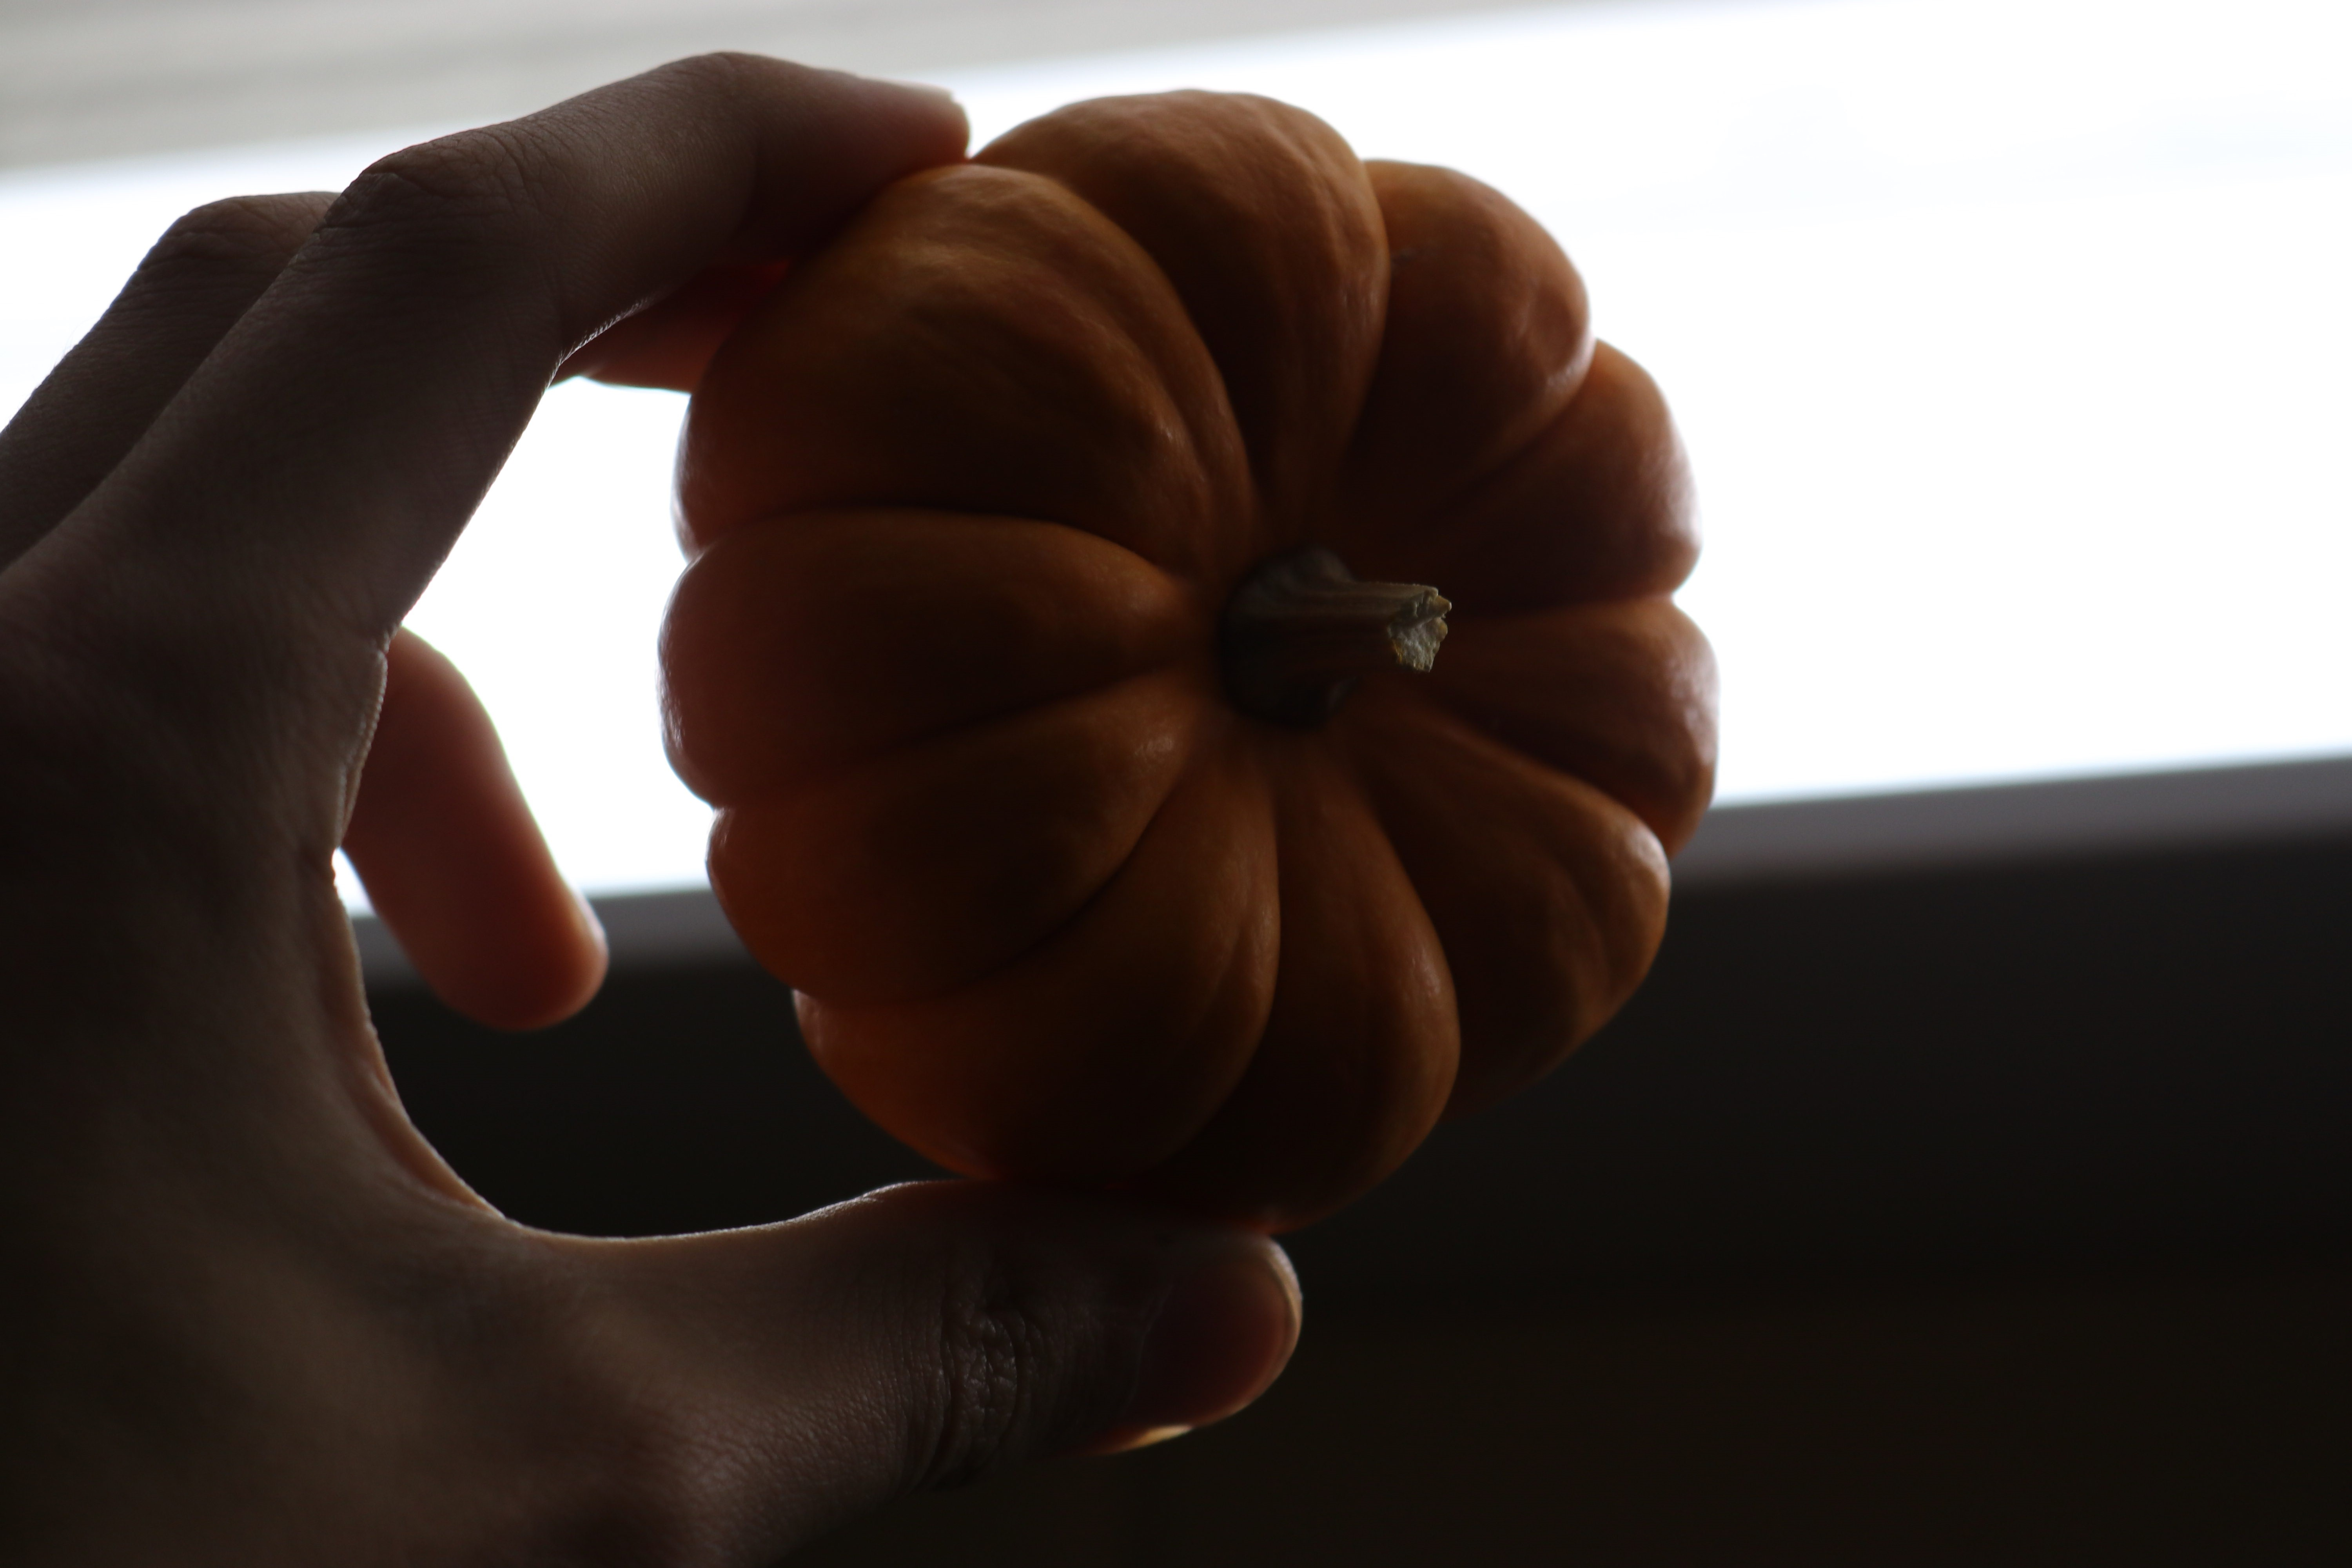
\includegraphics[width=8cm]{set3_pumpkin1.JPG}
			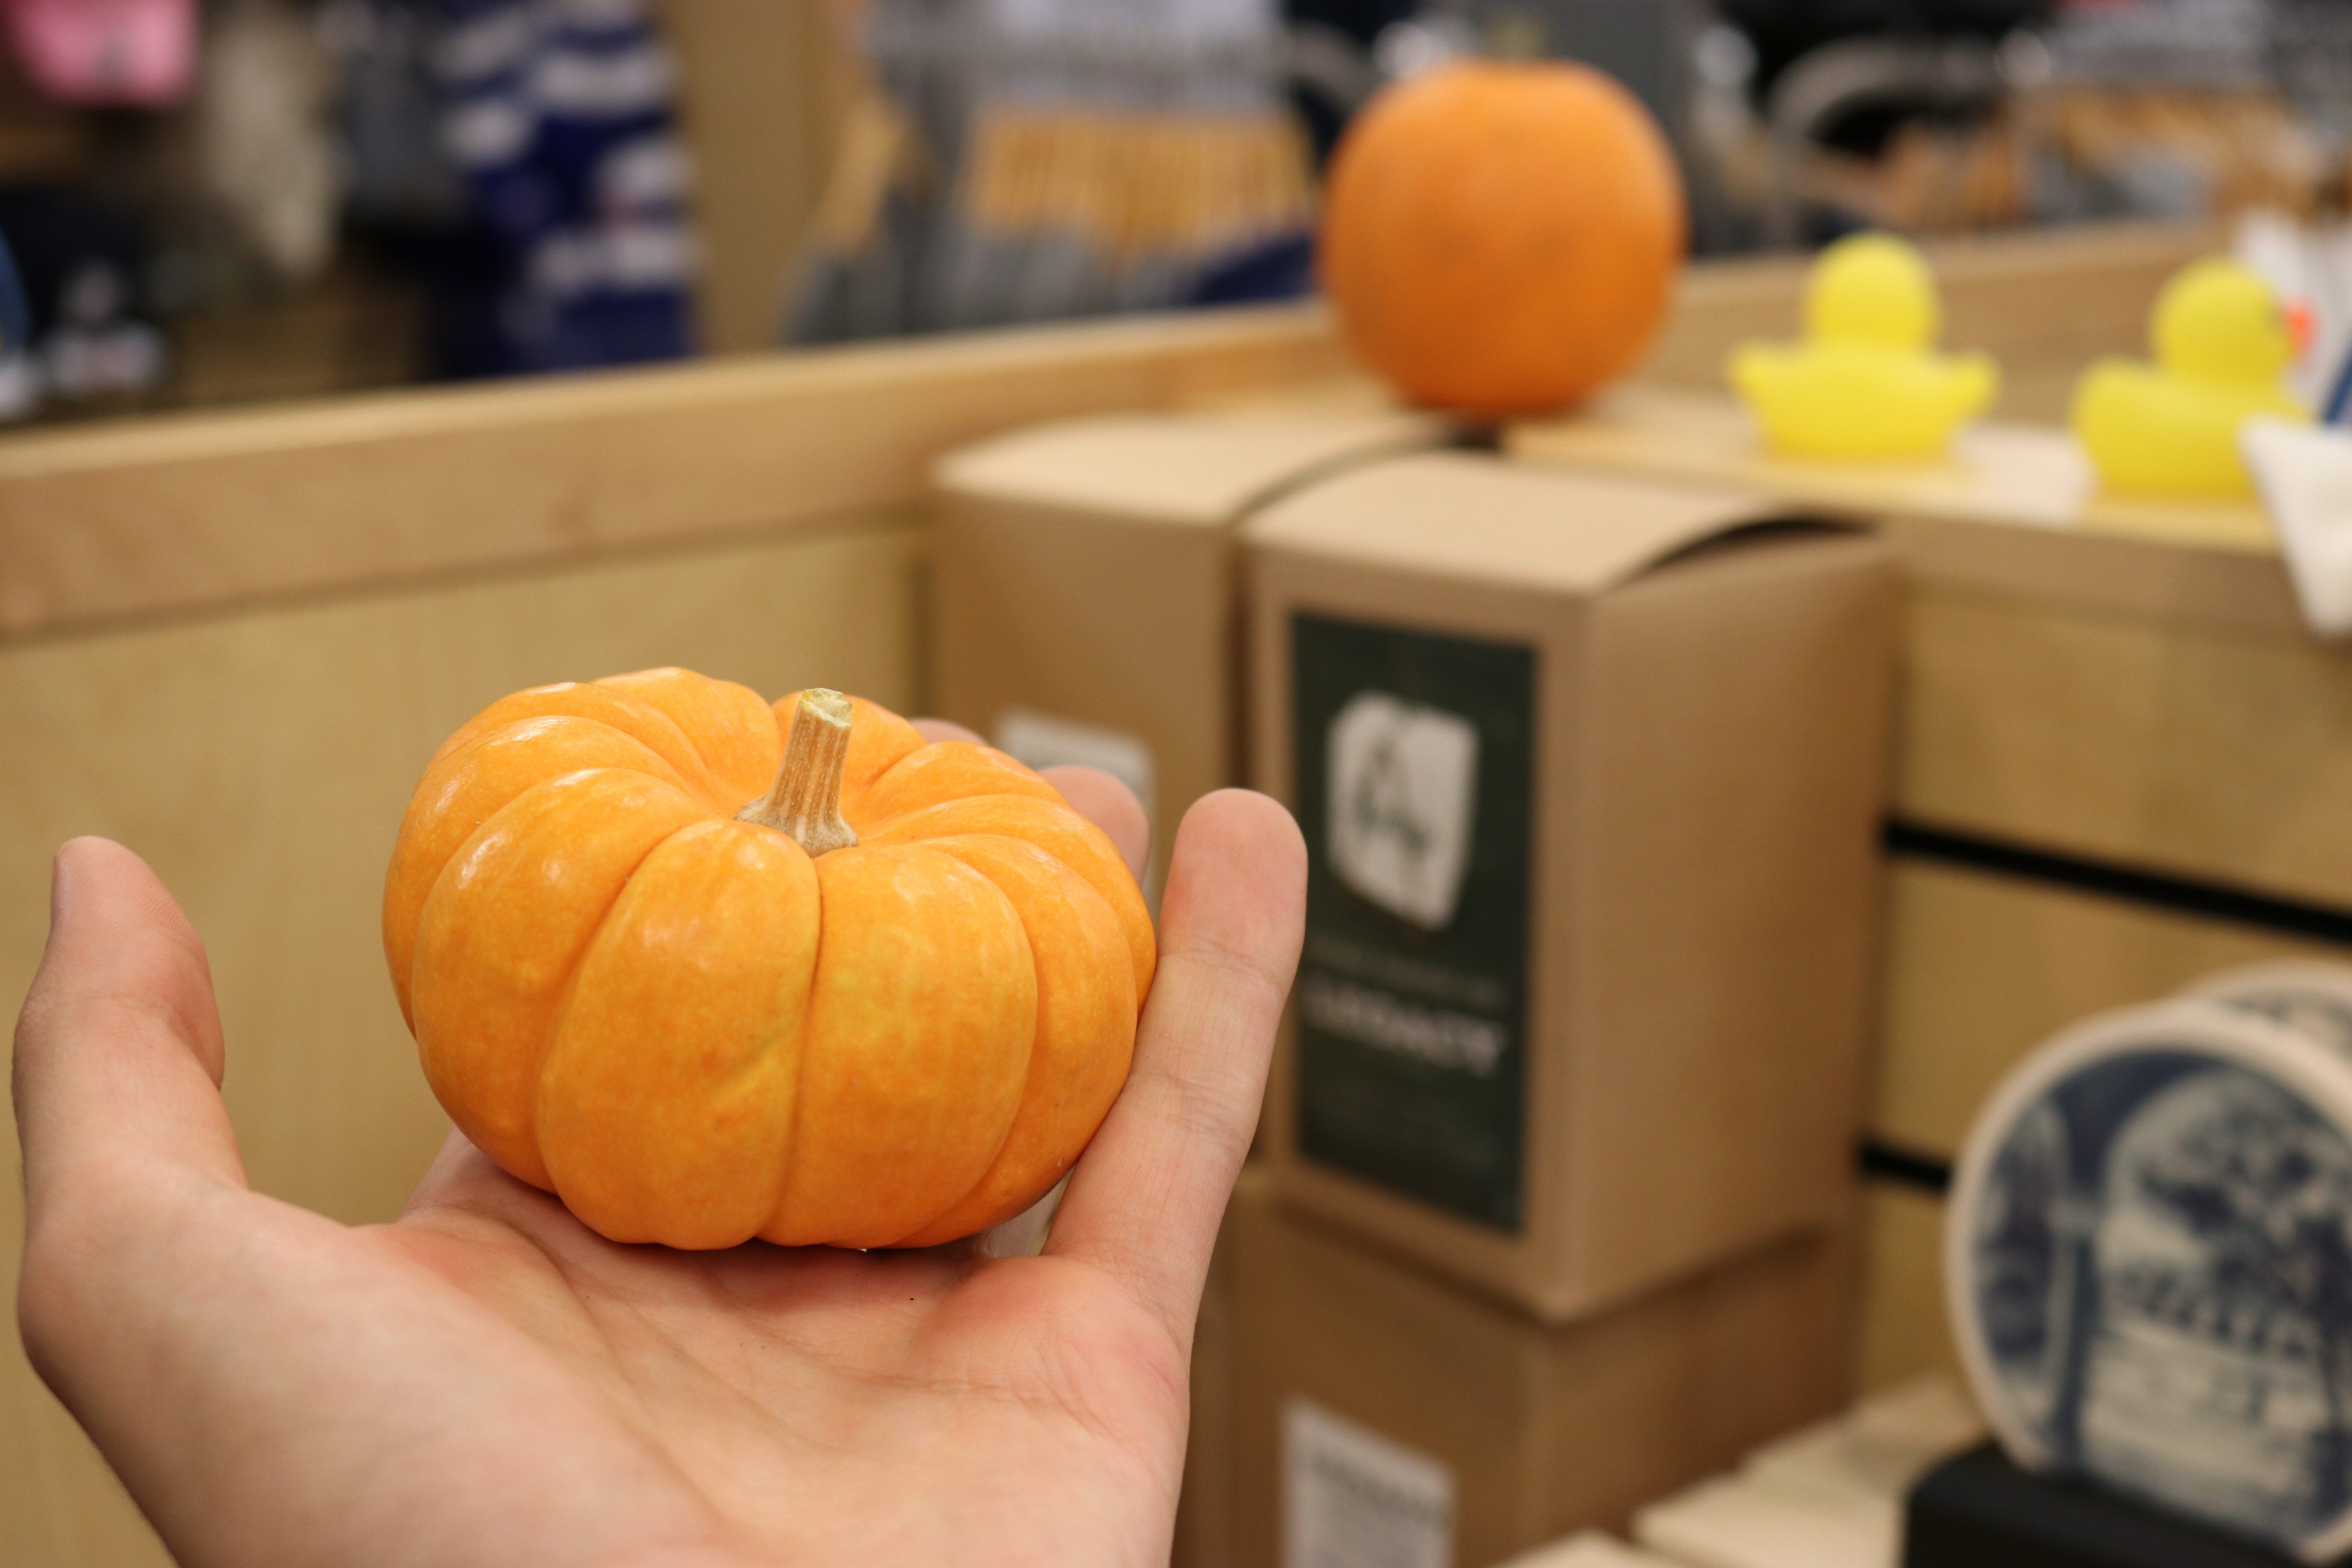
\includegraphics[width=8cm]{set3_pumpkin2.JPG}
			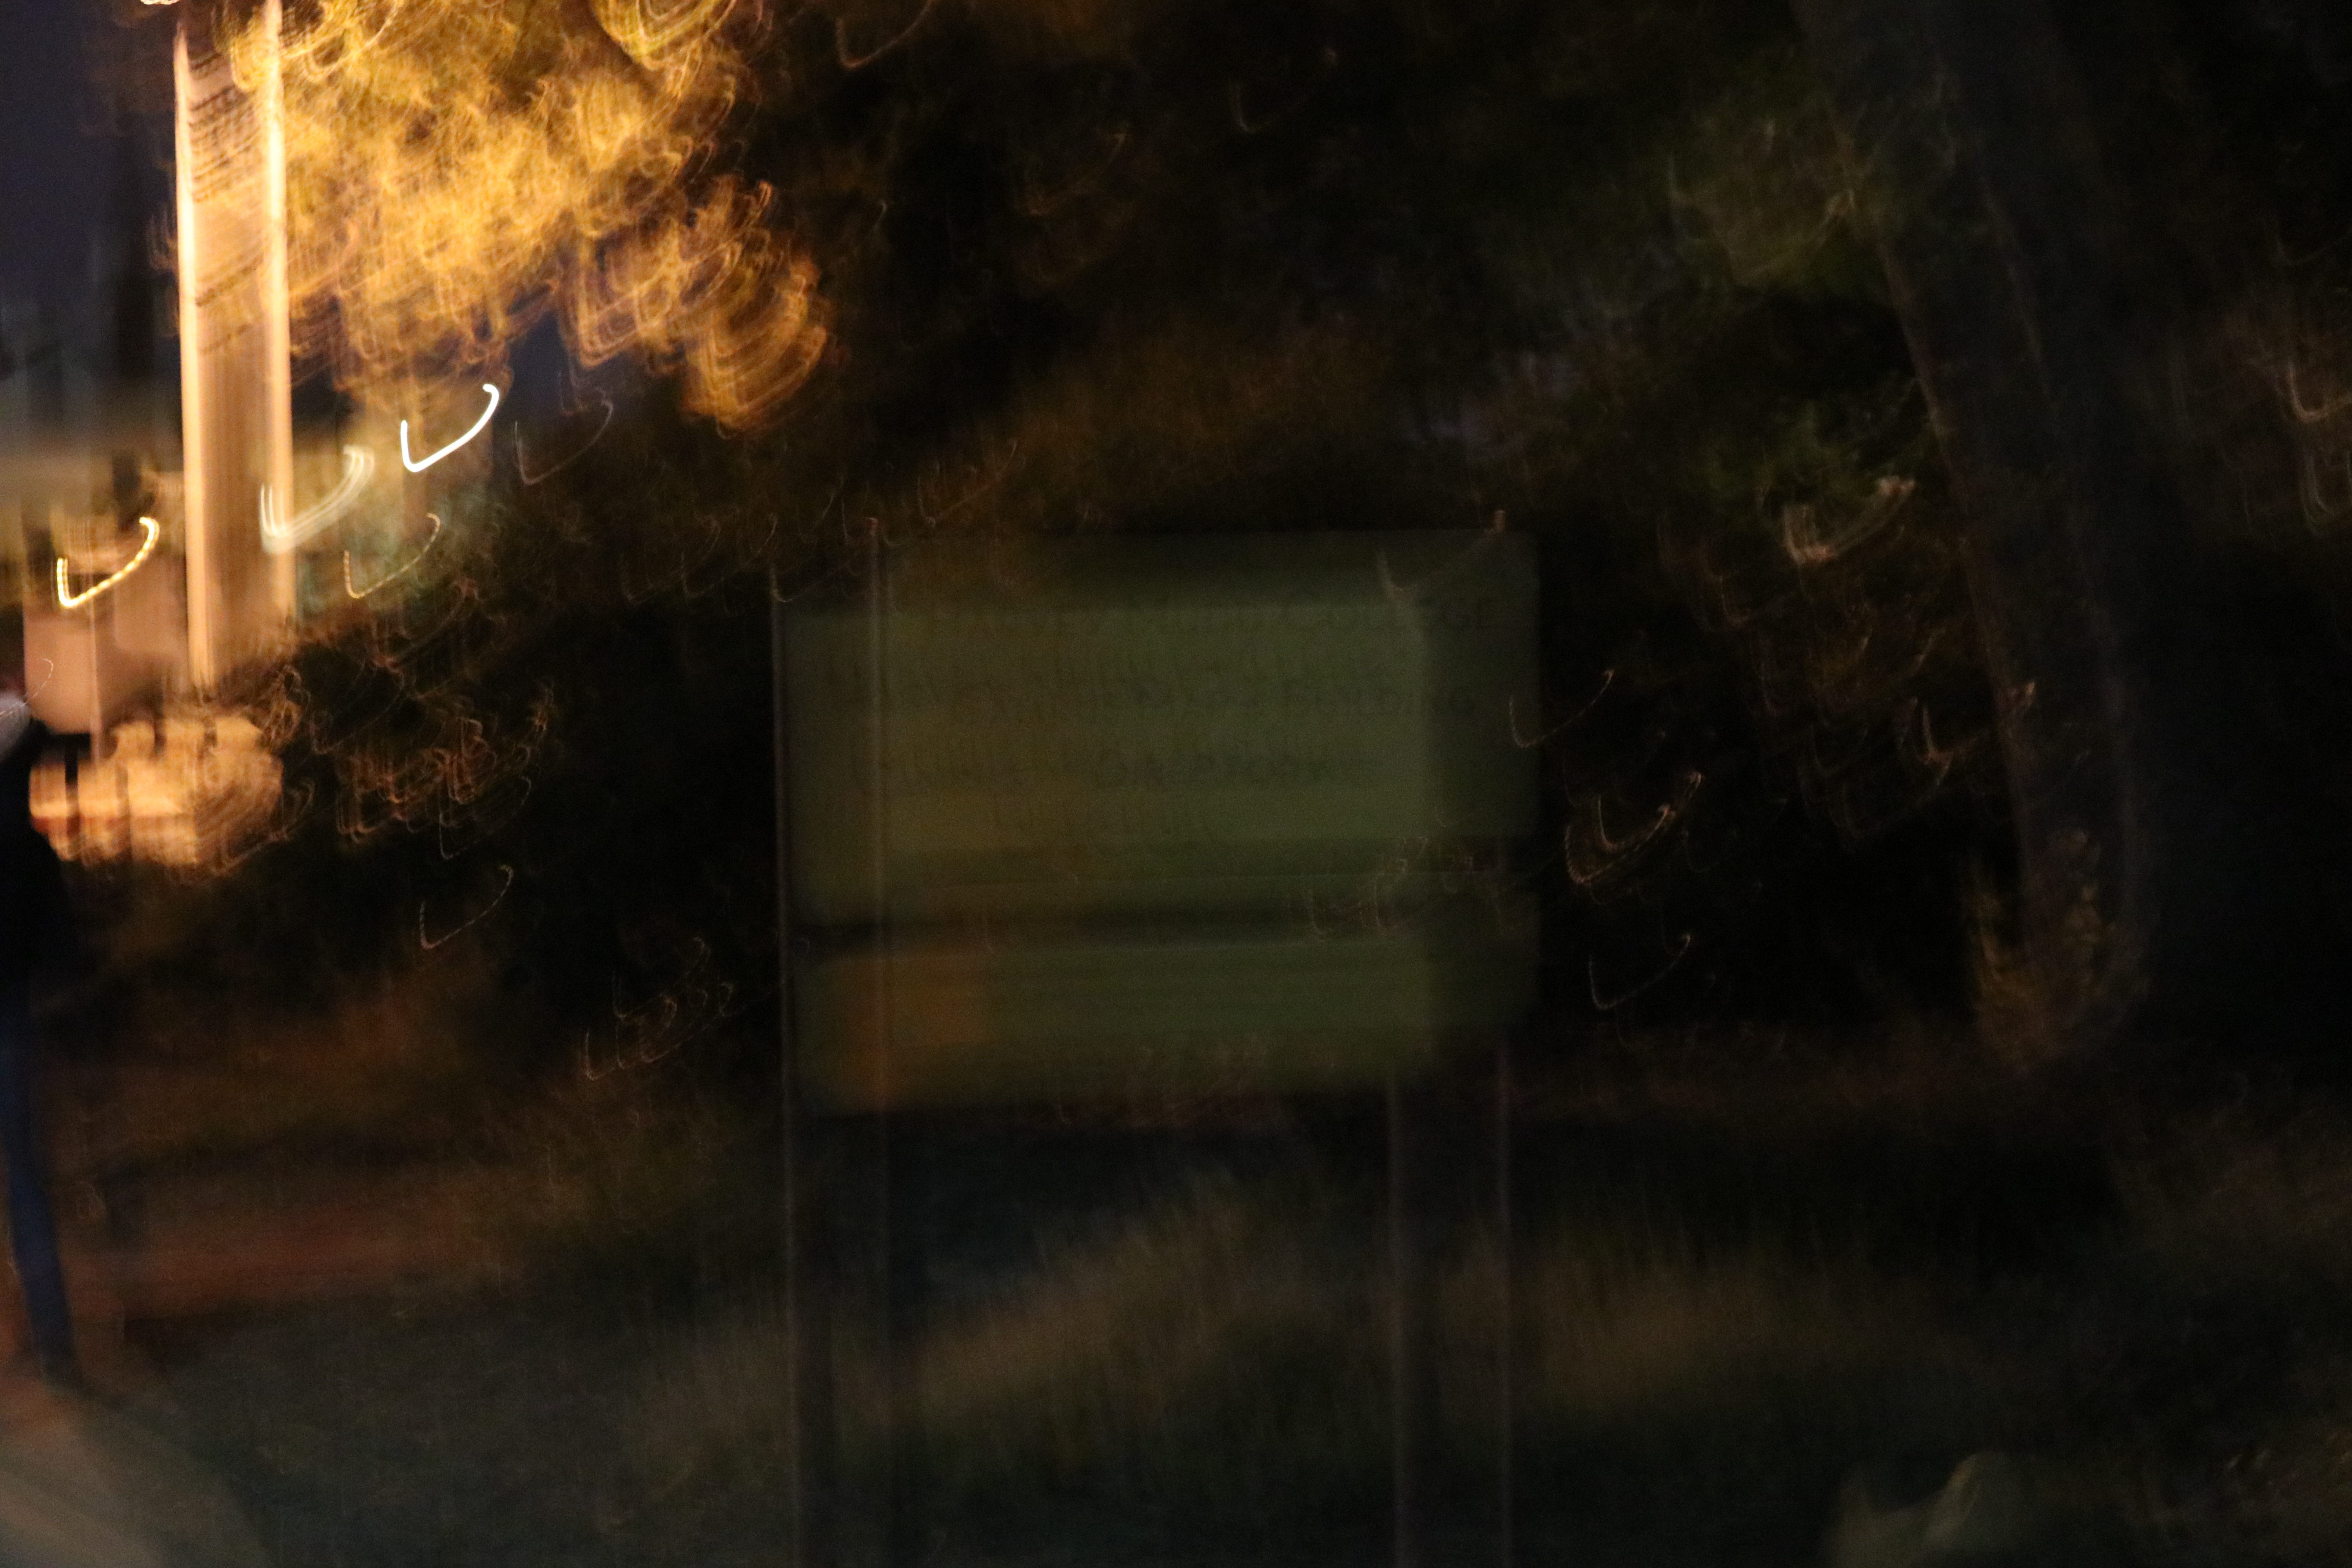
\includegraphics[width=8cm]{set3_other.JPG}
		\end{center}
	\end{figure}	
		
	\section{Experimental Design}
		The team had two goals in pipeline testing: to ensure that it was possible for the open-source DCraw engine to provide acceptable recognition rates (90\%+), and to minimize the number and complexity of image processing steps required to achieve these recognition rates.
		\subsection{Overall Parameter Testing}
		The first step in this investigation was to examine whether the DCraw engine can match the Inception-V3 binary recognition rate of the integrated camera ISP, and, if so, the parameter distribution required to do so.
		
		For each image set, 47 converted sets were generated by UFraw, each with a different set of parameter distributions. The settings of each UFraw parameter are shown in Figure \ref{ufraw_settings}, with all parameters not described by the given settings left at their defaults, such that an image set exists for every parameter value. A parameter description can be seen on the UFraw man page\footnote{https://www.freebsd.org/cgi/man.cgi?query=ufraw\&manpath=FreeBSD+Ports+7.0-RELEASE}.
		
		\begin{figure}
			\begin{center}
				\label{ufraw_settings}
				\caption{UFraw Parameter Test Settings}
				\begin{tabular}{cccccc}
					temperature & green & gamma & exposure & saturation & black-point \\
					2700 & 0.2 & 0.1 & -3 & 0 & 0 \\
					3000 & 0.6 & 0.3 & -2 & 1 & 0.2 \\
					3300 & 1 & 0.5 & -1 & 2 & 0.4 \\
					3600 & 1.4 & 0.7 & 0 & 3 & 0.6 \\
					3900 & 1.8 & 0.9 & 1 & 4 & 0.8 \\
					4200 & 2.2 && 2 & 5 & 1 \\
					4500 &&& 3 & 6 & \\
					4800 &&&& 7 & \\
					5100 &&&& 8 & \\
					5400 &&&&& \\
					5700 &&&&& \\
					6000 &&&&& \\
					6300 &&&&& \\
				\end{tabular}	
			\end{center}
		\end{figure}
	
		A full parameter command list is available in Section \ref{ufrawcommands}.
		
		After image set generation was completed, the Tensorflow test pipeline scripts in Section \ref{pipelinecode} were used to generate output metrics for each set of UFraw parameters.
		
		\subsection{Pipeline Step Testing}
		After image generation via UFraw, the team's next goal was to minimize the pipeline steps required to achieve adequate recognition rates. These tests were run without the UFraw frontend, as the raw DCraw engine provides much more control over applied ISP steps.
		
		
		The team first eliminated all DCraw steps requiring external files, such as dark frame correction. As shown in the previous parameter testing, DCraw conversion pipeline is capable of producing images with adequate recognition rates without these image processing steps. 
		
		The condensed DCraw pipeline is shown in Figure \ref{condenseddcraw}. These tests were run on the third image set with keyword squash.
		
		\begin{figure}
			\begin{center}
				\label{condenseddcraw}
				\caption{DCraw Pipeline}
				\begin{tabular}{lll}
					Conversion Step & Algorithm Options & Command-Line Arguments\\
					\hline
					Decode raw data & camera-specific & n/a\\
					Set up gamma curve & universal & n/a\\
					White balancing & auto & -a\\
					& camera statistics & -w\\
					& default statistics & n/a \\
					& none & -r 1 1 1 1 \\
					Colorspace conversion calculation & camera-specific & n/a\\
					Wavelet noise removal & universal & -n \\
					Color scaling & universal & n/a \\
					Interpolation & bilinear & -q 0 \\
					& VNG & -q 1 \\
					& PPG & -q 2 \\
					& AHD & -q 3 \\
					Highlight reconstruction & Clip all & -H 0 \\
					& Leave unclipped & -H 1 \\
					& Blend highlights & -H 2 \\
					& Reconstruct highlights & -H 5 \\
				\end{tabular}
					
			\end{center}
		\end{figure}
		
	\section{Results and Data Analysis}
	\subsection{Overall Parameter Testing}
	While raw data is available in \ref{dcrawdata}, the relevant data can be seen in Figure \ref{overallgraphs}. It is clear that while parameter-recognition rate relationships differ between image sets, it is possible to achieve 90\%+ recognition rates through all image sets, and therefore fulfilled the required statistic.
	
	\begin{figure}
		\begin{center}
			\label{overallgraphs}
			\caption{Recognition Rate-Parameter Graphs}
			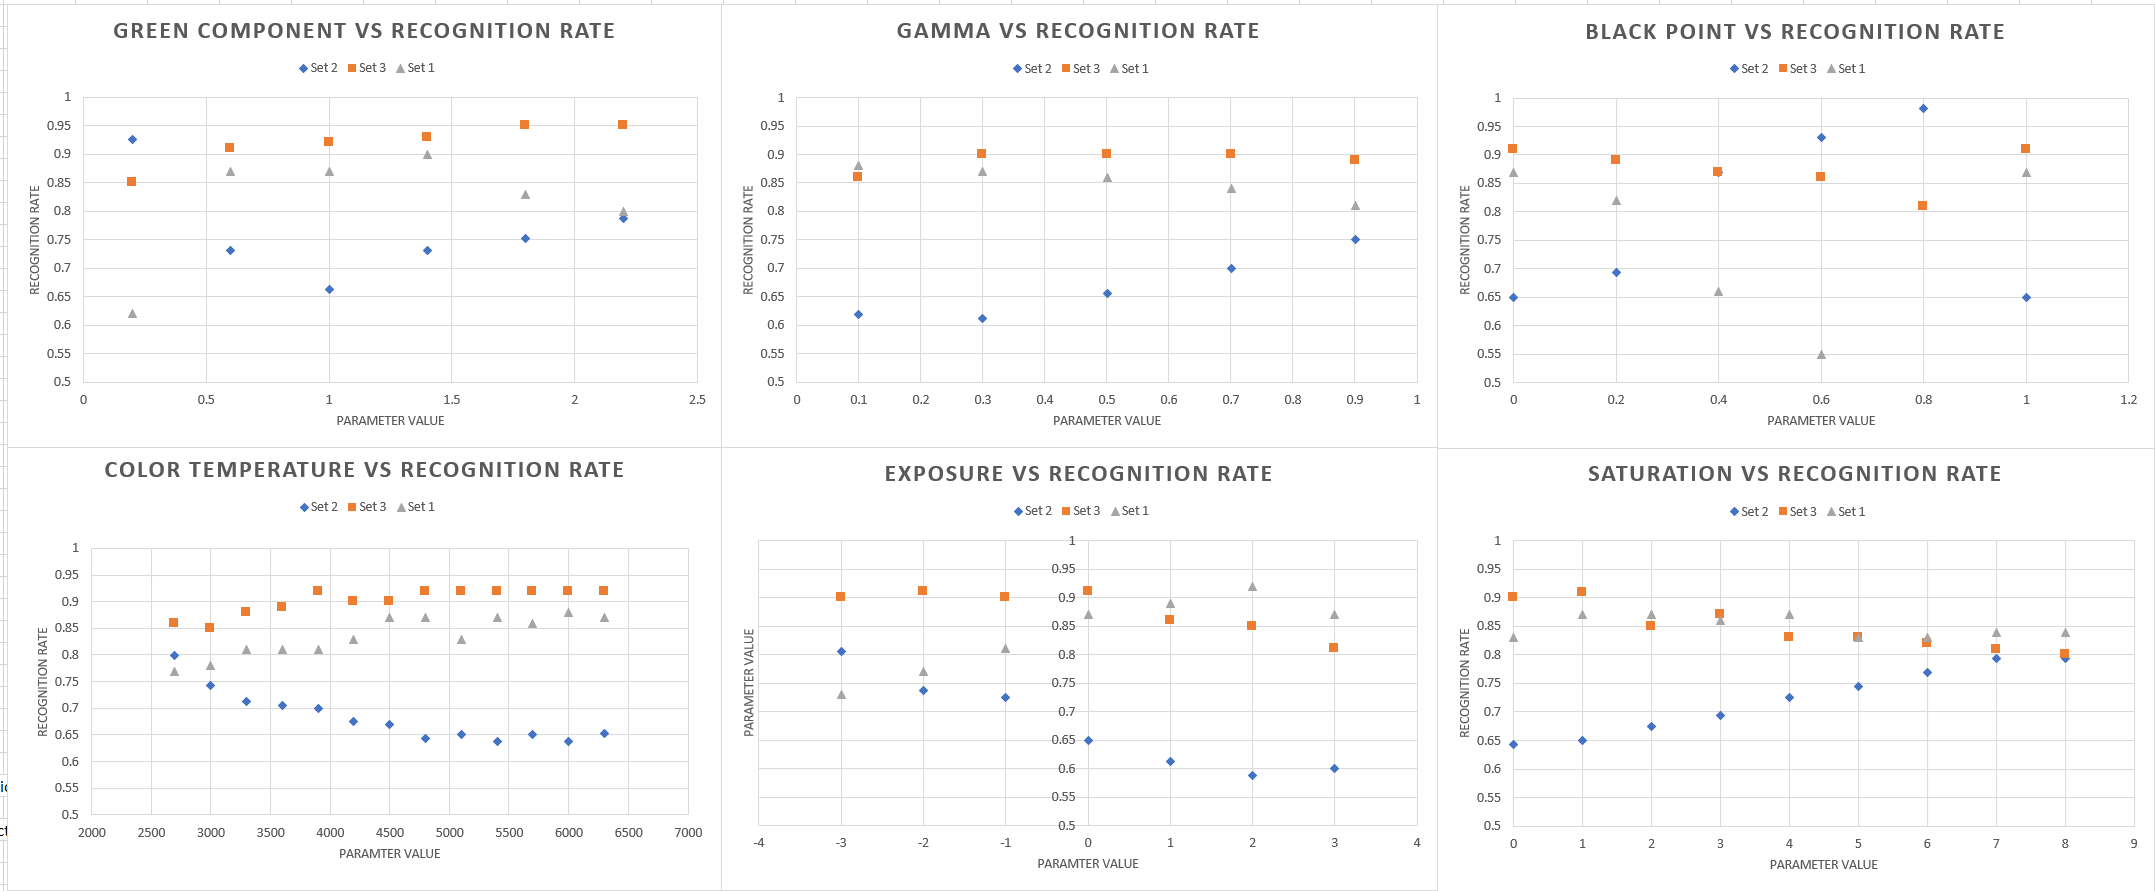
\includegraphics[scale=0.5]{all_graphs.png}
		\end{center}
	\end{figure}
	
	
	
	\subsection{Pipeline Step Testing}
	Raw data is available in Figure \ref{datapipeline}. All options provide similar percent recognition, all above the 90\% threshold. This indicates that for this image set it is possible to only implement the simplest algorithms in the hardware ISP: no white balancing, bilinear interpolation, no highlight reconstruction, and no denoising.
	
	\begin{figure}
		\begin{center}
			\label{datapipeline}
			\caption{DCraw Pipeline Statistics}
			\begin{tabular}{llcc}
				Conversion Step & Algorithm Options & Recognized Images & Percent Recognition \\
				White balancing & auto & 96 & 94.1\%\\
				& camera statistics & 93 & 91.1\%\\
				& default statistics & 94 & 92.2\%\\
				& none & 92 & 90.1\%\\
				Interpolation & bilinear & 93 & 91.1\%\\
				& VNG & 93 & 91.1\%\\
				& PPG & 93 & 91.1\%\\
				& AHD & 93 & 91.1\%\\
				Highlight Reconstruction & Clip all & 93 & 91.1\%\\
				& Leave unclipped & 93 & 91.1\%\\
				& Blend highlights & 93 & 91.1\%\\
				& Reconstruct highlights & 93 & 91.1\%\\
				Wavelet Noise Removal & No denoising & 93 & 91.1\%\\
				& 92 & 91.1\%
			\end{tabular}
		\end{center}
	\end{figure}
	
	\section{Conclusion}
	The data from both pipeline tests illustrated that it is feasible to base the hardware ISP off of the algorithms found in DCraw. Importantly, recognition rates past the 90\% threshold are possible by implementing only the simplest DCraw pipeline, allowing a simpler and more power and area efficient hardware design.

\chapter{Spring Plans}

\chapter{Appendix}

\section{DCRaw Test Data} \label{dcrawdata}

\section{Condensed DCraw Codebase}

\section{Verilog ISP Implementation}

\section{Tensorflow Testing Pipeline} \label{pipelinecode}

\section{UFraw Test Commands} \label{ufrawcommands}




\end{document}